\subsection{Frontend Arkitektur}

Front-end applikationen er det man kan kalde, brugerens vindue til spillet, det er i dette modul at brugeren vil få alt sit information og vil få mulighed for at lave inputs til spillet. Det er yderligere her at der skal tages hånd om brugerens input således at de rigtige funktioner i Game Enginen bliver kaldt når brugeren trykker på en vilkårlig knap.\\
Front-end'en er opbygget af et hav af forskellige skærme og menuer, og for at give et overblik over disse er der lavet følgende C3 model for Front-end'en (\autoref{fig:Arkitektur-FrontEnd-C3}), som giver en idé om hvilke skærme og menuer der kan gå til hvilke andre menuer/skærme. Udover dette fortæller modellen også om hvordan og hvilke skærme og menuer der snakker med noget uden for Front-end'en selv f.eks. skal der ved Login/Register kontaktes databasen for at få verificeret logind-oplysninger, og samtidig skal der ved save og load-game hentes en liste af gemte spil i databasen hvorefter der skal henholdsvis skrives og hentes fra databasen alt efter om man gemmer eller henter et spil. Der skal hertil nævnes at Login og Register står til at snakke med backenden direkte og ikke igennem gamelogic blokken, dette er valgt da funktionen ikke kaldes i gamelogic blokken, men den kaldes direkte i backend controlleren. Derudover er modellen mere overskuelig på denne måde og fungerer bedre til at give overblik over navigationen igennem menuerne.

\begin{figure}[H]
\centering
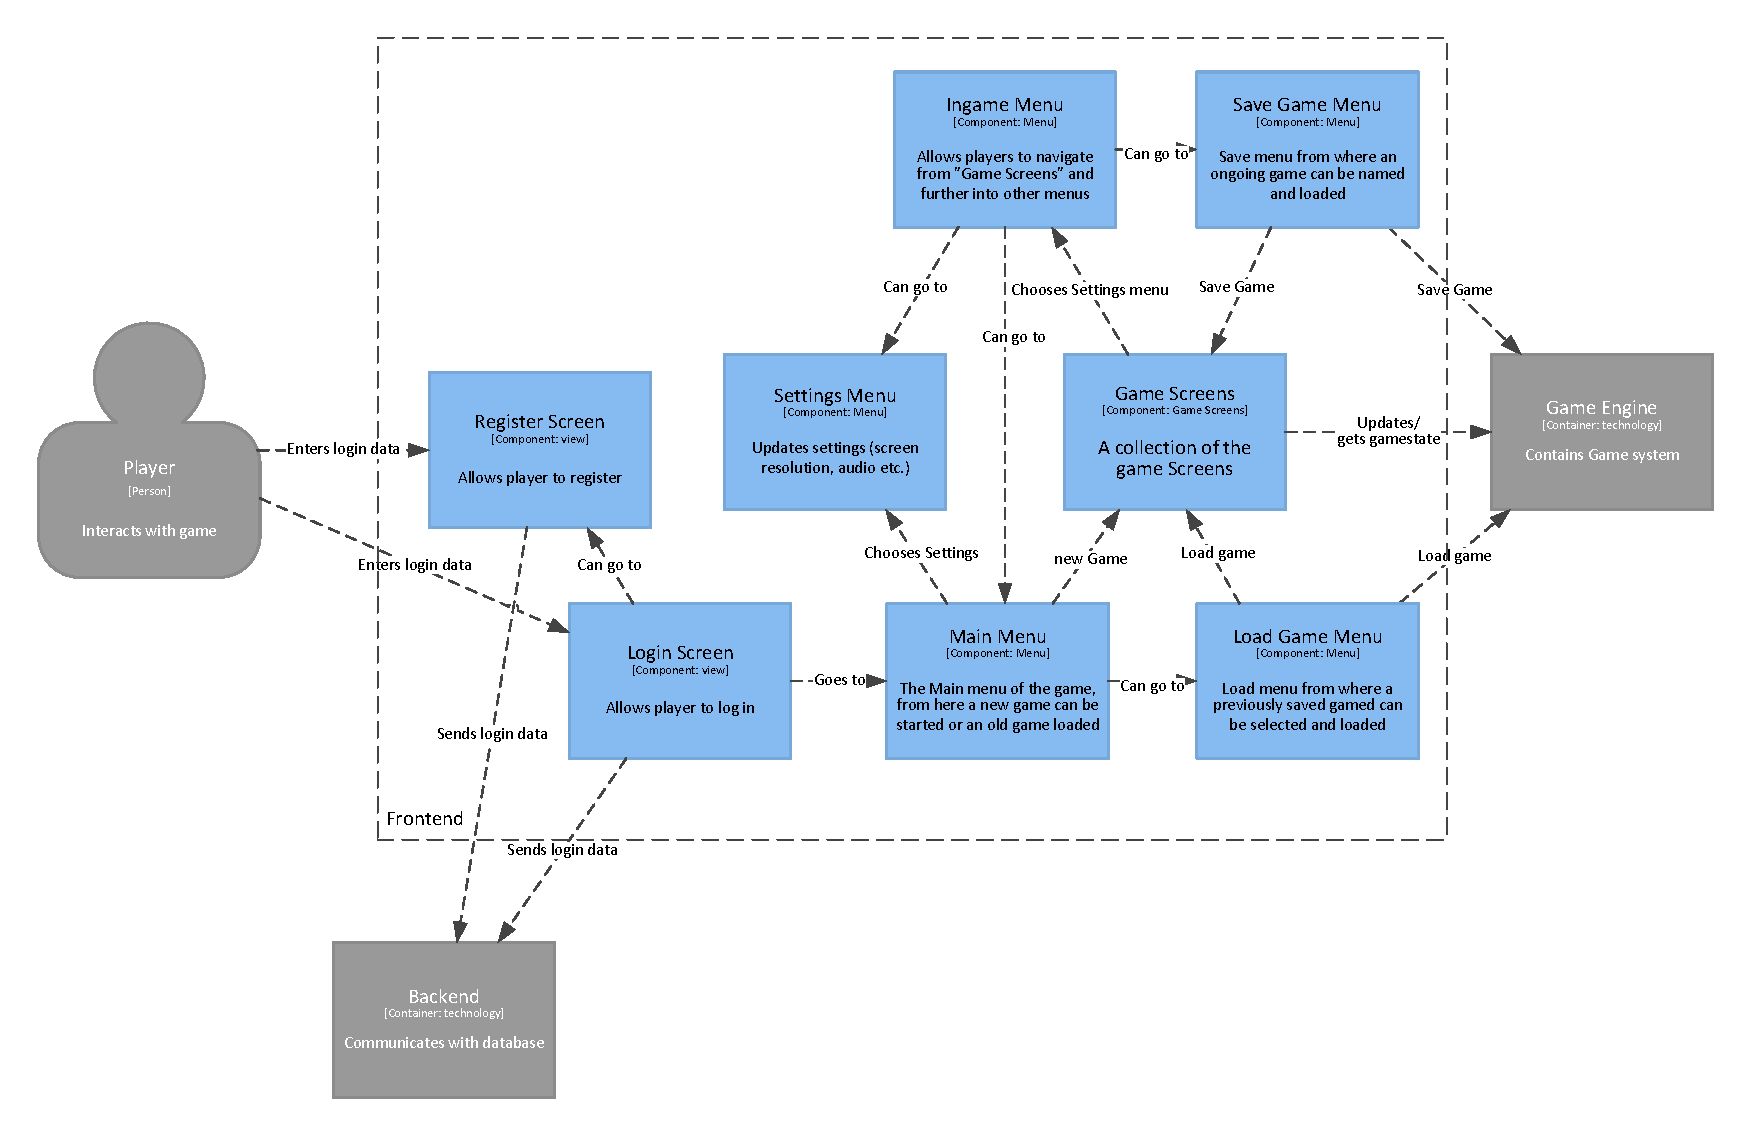
\includegraphics[width = \textwidth]{02-Body/Images/Frontend_C3.pdf}
\caption{C3-Model for Frontend. Modellen fortæller hvordan man kan navigere igennem forskellige menuer og hvilke menuer der kan føre til hvad. Derudover kan man se hvilke blokke der snakker ud af frontenden og sammen med resten af systemet.}
\label{fig:Arkitektur-FrontEnd-C3}
\end{figure}

\subsubsection{Pseudo Frontend Arkitektur}
For at give overblik over, hvordan kommunikationen mellem frontend, backend og gamecontroller kommer til at foregå, er der lavet et pseudo sekvensdiagram for følgende UserStories:
\\
- Login\\
- Register\\
- Save Game\\
- Load Game\\

Der vil i dette afsnit kun blive vist "Save Game". "Load Game","Login" og "Register" kan findes i Tekniskbilag \textbf{(INDSÆT REFERENCE HER)}.

\noindent På \autoref{fig:Arkitektur-FrontEnd-Save} ses "Save Game", som viser forløbet når en bruger gerne vil gemme sit igangværende spil, set fra Frontends perspektiv. Her kan man bide mærke i, at når der skiftes skærm, vil den nye skærm få initialiseret sine variabler i sin constructor og derfor er der kun et selvkald, hver gang skærmen skiftes. Dette selvkald tager hånd om at opdatere mappen således at spilleren er i det rigtige rum, og at man kun kan se det af mappen, man har været i.
Hertil skal der nævnes at hvis brugeren er i "Combat State" er det ikke muligt at gemme spillet og knappen "Save Game" på "In Game Menu" vil ikke kunne ses eller bruges.\\

\begin{figure}[H]
\centering
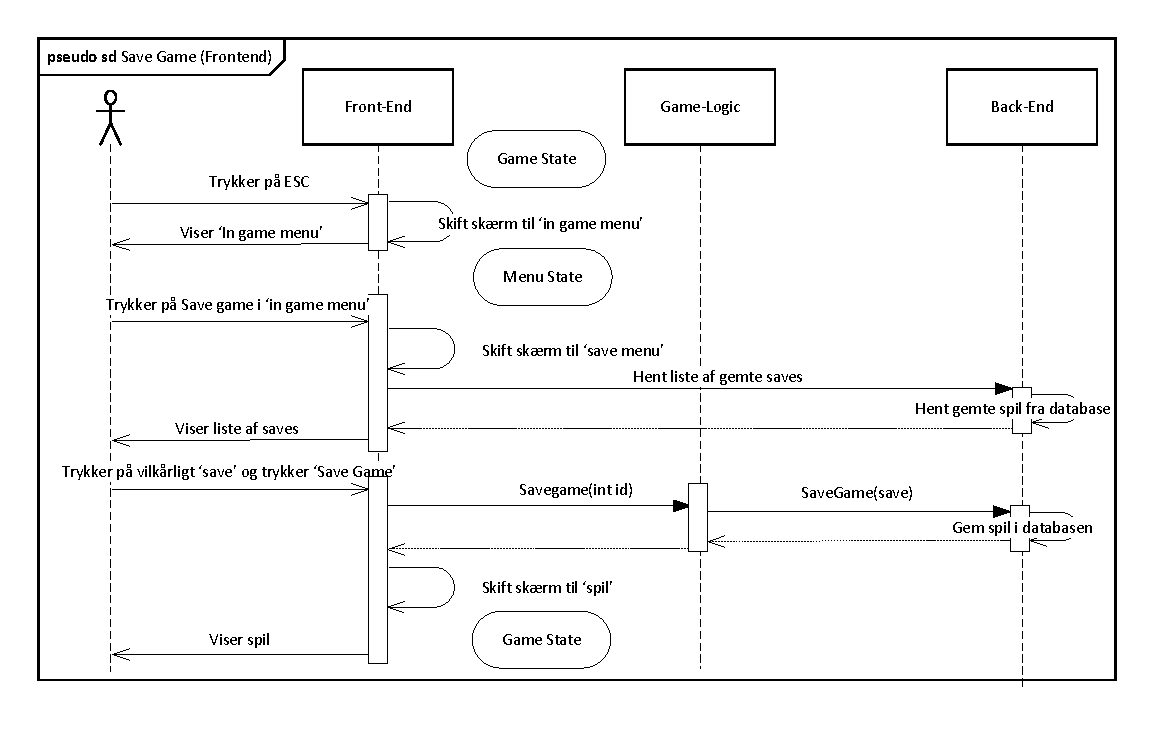
\includegraphics[width = \textwidth]{02-Body/Images/Front-End_-_Arkitektur-savegame.pdf}
\caption{Pseudo sekvensdiagram af forløbet af userstory "Save Game", set fra Frontends perspektiv. Der laves 2 kald til databasen igennem Backenden, hvori der i det første kald,  "Hent liste af gemte saves" hentes en liste af brugerens gemte spil og i andet kald gemmes brugerens nuværende spil henover det valgte spil.}
\label{fig:Arkitektur-FrontEnd-Save}
\end{figure}

\newpage
